\documentclass[a4paper]{article}

% Packages
\usepackage[14pt]{extsizes}
\usepackage[T2A]{fontenc}
\usepackage[russian]{babel}
\usepackage[left=20mm, top=15mm, right=15mm, bottom=20mm]{geometry}
\usepackage{graphicx} % For images
\usepackage{amsmath, amssymb} % For equations
\usepackage{booktabs} % For better tables
\usepackage{pgfplots} % For plotting graphs
\usepackage{xcolor} % For color support
\usepackage{caption} % For captioning tables and figures
\usepackage{float} % For precise float placement (images, tables)
\usepackage{array} % For better table management
\usepackage[hidelinks]{hyperref} % For table of contents to be clickable
\usepackage{bookmark}
\usepackage{multirow}
\usepackage{array}
\usepackage{cancel}
\usepackage{placeins}
\usepackage{enumitem}
\pgfplotsset{compat=1.17}

% Importing custom definitions (lstset, tikzset, etc.)
\newcommand{\labtitle}[9]{
	\begin{center}
		\vspace*{-1.8cm}
		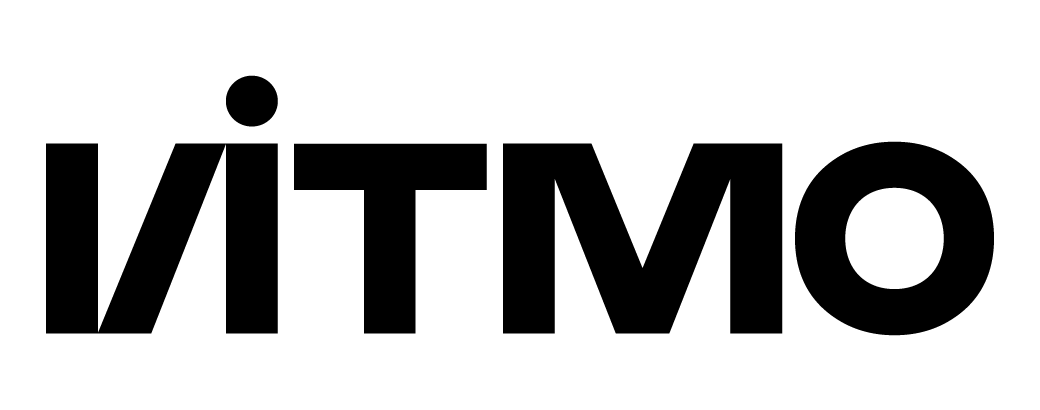
\includegraphics[width=0.26\textwidth]{../common/itmo-logo.png}\\
		\vspace{2.4cm}
		\textbf{\Large Основы электротехники}\\[1.2cm]
		\textbf{\Large Отчёт по лабораторной работе №#1}\\[0.7cm]
		\textbf{\Large #2}\\[3cm]

		\textbf{\Large Группа \textcolor{red}{\textit{P#3}}}\\[0.2cm]
		\textbf{\Large Вариант \textcolor{red}{\textit{#4}}}\\[3cm]

		\begin{flushleft}
			\textbf{\large Выполнил: \textcolor{red}{\textit{#5}}}\\[0.5cm]
			\textbf{\large Дата сдачи отчёта: \textcolor{red}{#6}}\\[0.5cm]
			\textbf{\large Дата защиты: \textcolor{red}{#7}}\\[0.5cm]
			\textbf{\large Контрольный срок защиты: \uline{#8}}\\[0.5cm]
			\textbf{\large Количество баллов: \uline{#9}}\\[2cm]
		\end{flushleft}
	\end{center}

	\vspace*{\fill}
	\begin{center}
		\textbf{\Large СПб -- 2024}
	\end{center}
	\vspace*{-1.8cm}
}

\newcommand{\hwtitle}[8]{
	\begin{center}
		\vspace*{-1.8cm}
		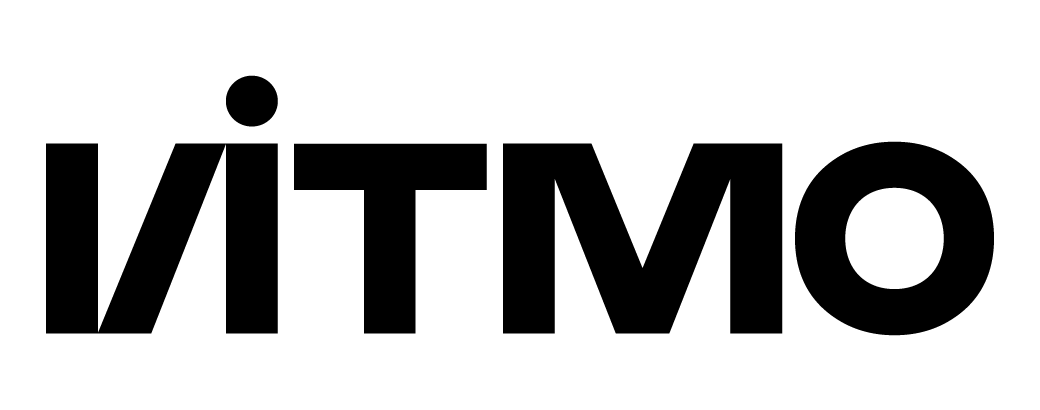
\includegraphics[width=0.26\textwidth]{../common/itmo-logo.png}\\
		\vspace{2.4cm}
		\textbf{\Large Основы электротехники}\\[1.2cm]
		\textbf{\Large Домашнее задание №#1}\\[0.7cm]
		\textbf{\Large #2}\\[3cm]

		\textbf{\Large Группа \textcolor{red}{\textit{P#3}}}\\[0.2cm]
		\textbf{\Large Вариант \textcolor{red}{\textit{#4}}}\\[3cm]

		\begin{flushleft}
			\textbf{\large Выполнил: \textcolor{red}{\textit{#5}}}\\[0.5cm]
			\textbf{\large Дата сдачи: \textcolor{red}{#6}}\\[0.5cm]
			\textbf{\large Контрольный срок сдачи: \uline{#7}}\\[0.5cm]
			\textbf{\large Количество баллов: \uline{#8}}\\[2cm]
		\end{flushleft}
	\end{center}

	\vspace*{\fill}
	\begin{center}
		\textbf{\Large СПб -- 2024}
	\end{center}
	\vspace*{-1.8cm}
}



% -------------------------------

\begin{document}

% Title page
\labtitle{2}{Исследование переходных процессов в электрических цепях}{3331}{9}{Дворкин Борис Александрович}{07.10.2024}{09.10.2024}{09.10.2024}{}
\thispagestyle{empty}

\newpage
\pagestyle{plain}
\setcounter{page}{1}

% -------------------------------

% autogenerated table of contents
\linespread{0.9}
\tableofcontents
\linespread{1}

% -------------------------------

\newpage
\section*{Цель работы}
\addcontentsline{toc}{section}{Цель работы}

Исследование переходных процессов в электрических цепях первого и
второго порядков с источником постоянного и переменного напряжения.

% -------------------------------

\section*{Часть 1}
\addcontentsline{toc}{section}{Часть 1}
\stepcounter{section}
\subsection{Исследование RC-цепи}

\subsubsection{Схема исследуемой цепи}
На рисунке 1.1 представлена схема замещения генератора прямоугольного напряжения с резистивной и ёмкостной нагрузкой, созданная в приложении LTspice.

\begin{figure}[H]
	\centering
	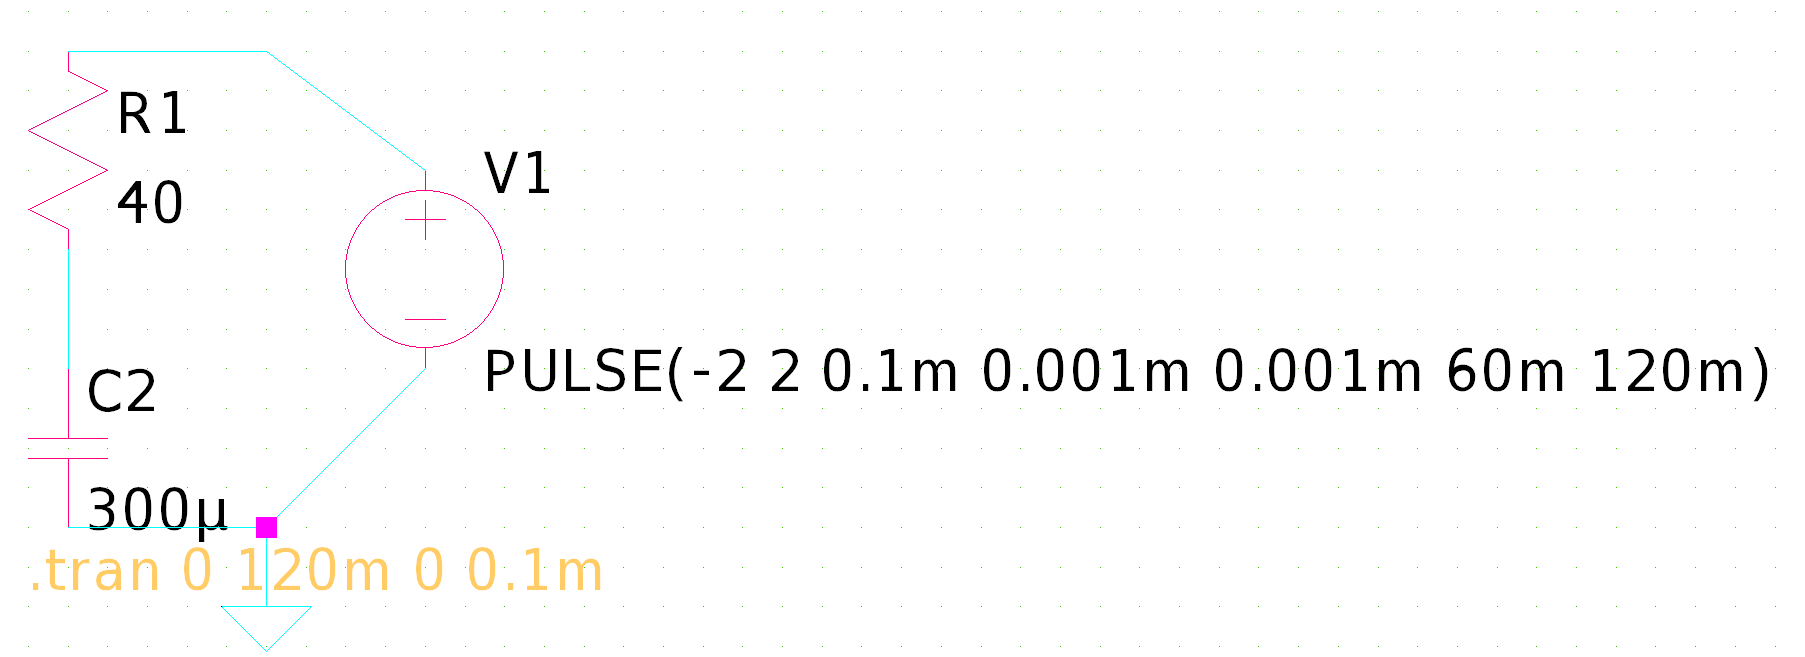
\includegraphics[width=1\textwidth]{./data/rc-schema.png}
	\caption{Схема замещения RC-цепи в LTspice.}
\end{figure}

\subsubsection{Расчётные формулы и расчёты}
\begin{enumerate}
	\item \textbf{Постоянная времени } $\tau$ \textbf{в RC-цепи} рассчитывается по формуле:

	      \[
		      \tau = R \cdot C
	      \]

	      где $R = 40 \, \Omega$ и $C = 300 \, \mu F$.

	      Подставим значения:

	      \[
		      \tau = 40 \, \Omega \cdot 300 \cdot 10^{-6} \, F \cdot 10^{-3} = 12 \, \text{мс}
	      \]

	\item Расчётные значения тока и напряжения на конденсаторе после коммутации, а также установившиеся значения напряжения на конденсаторе и тока в цепи для RC-цепи рассчитываются по следующим формулам:

	      \[
		      \lim_{t \to 0^+} U_C(t) = \lim_{t \to 0^-} E(t) = -2 \, \text{В}
	      \]

	      \[
		      \lim_{t \to 0^+} I(t) = \frac{E + U_C}{R} = \frac{2\, \text{В} + 2\, \text{В}}{40 \, \Omega} = 100 \, \text{мА}
	      \]

	      \[
		      \lim_{t \to \infty} I(t) = \lim_{t \to 0^-} I(t) = 0 \, \text{мА}
	      \]

	      \[
		      \lim_{t \to \infty} U_C(t) = \lim_{t \to 0^+} E(t) = 2 \, \text{В}
	      \]

	\item Значение времени переходного процесса \( t_{0.5} \) определяется как время, за которое ток достигает \textit{половины} своего амплитудного значения. Постоянная времени \( \tau \) определяется как:

	      \[
		      \tau = \frac{t_{0.5}}{\ln 2}
	      \]

	      \textbf{Вычисление постоянной времени } \( \tau \):

	      \[
		      \tau = \frac{t_{0.5_I}}{\ln 2} = \frac{8.418554 \, \text{мс}}{0.69314718} = 12.144 \, \text{мс}
	      \]

\end{enumerate}

Постоянная времени \( \tau \) была определена экспериментально и составляет \( 12.144 \, \text{мс} \). Это значение будет использовано для расчёта соответствующих токов и напряжений в цепи.


\subsubsection{График переходного процесса в RC-цепи}
% lab2.txt data structure:
% time	V(n001)	V(n002)	I(R1)

\begin{figure}[h]
	\centering
	\begin{tikzpicture}[scale=0.88]

		% Voltage axis
		\begin{axis}[
			width=17cm, height=12cm,
			xlabel={Время [мс]},
			ylabel={Напряжение [В]},
			grid=major,
			legend style={at={(0.857,0.95)}, anchor=north west},
			thick,
			xmin=0, xmax=120,
			ymin=-2, ymax=2,
			axis y line=right,
			axis x line=bottom,
			label style={font=\small},
			tick label style={font=\small},
			major tick length=0.2cm,
			ytick style={thick, black},
			xtick style={thick, black},
			ytick={-1.6, -1.2, -0.8, -0.4, 0, 0.4, 0.8, 1.2, 1.6},
			extra y ticks={-2, 2},
			extra y tick style={tick style={opacity=0}},
			x unit=0.001,
			]

			% Plot V(n001)
			\addplot[
				color=red,
				line width=1.2pt,
			] table [x expr=\thisrowno{0}*1000, y index=1, col sep=space] {./data/lab2.txt};
			\addlegendentry{$E$}

			% Plot V(n002)
			\addplot[
				color=green,
				line width=1.2pt,
				% nodes near coords,
				% mark=*,
				% every node near coord/.append style={font=\tiny, black}
			] table [x expr=\thisrowno{0}*1000, y index=2, col sep=space] {./data/lab2.txt};
			\addlegendentry{$U_c$}

			\draw[dashed,grey,very thin] (axis cs:120,1.972884) -- (axis cs:60.1,1.972884);
			\addplot[color=black, only marks, mark=*, mark size=2pt] coordinates {(60.1,1.972884)};
			\node[anchor=west] at (axis cs:60.1,1.872884) {\scriptsize $U_c(\infty) = 1.973 \, \text{В}$};

			\draw[dashed,grey,very thin] (axis cs:120,-1.973) -- (axis cs:120, -1.973)
			\addplot[color=black, only marks, mark=*, mark size=2pt] coordinates {(120, -1.973)};
			\node[anchor=east] at (axis cs:121,-1.82) {\scriptsize $ -1.973 \, \text{В} = U_c(0+)$};

		\end{axis}

		% Current axis
		\begin{axis}[
			width=17cm, height=12cm,
			xmin=0, xmax=120,
			ymin=-100, ymax=100,
			axis y line=left,
			axis x line=none,
			thick,
			ylabel={Ток [мА]},
			label style={font=\small},
			tick label style={font=\small},
			major tick length=0.2cm,
			ytick style={thick, black},
			ytick={-80, -60, -40, -20, 0, 20, 40, 60, 80},  % Y-axis ticks without ymax
			extra y ticks={-100, 100}, % Add min and max ticks for right axis
			extra y tick style={tick style={opacity=0}}, % Hide tick marks for these
			legend style={at={(0.955,0.82)}, anchor=north east}, % Legend position for Current
			]
			% Plot I(R1)
			\addplot[
				color=blue,
				line width=1.2pt,
				% mark=ball,
				% mark size=1.5pt
			] table [x expr=\thisrowno{0}*1000, y expr=\thisrowno{3}*1000, col sep=space] {./data/lab2.txt};
			\addlegendentry{$I$}

			\addplot[color=black, only marks, mark=*, mark size=2pt] coordinates {(0.13, 100)};
			\node[anchor=west] at (axis cs:0,95.5) {\scriptsize $I(0+) = 99.996 \, \text{мА}$};

			\addplot[color=black, only marks, mark=*, mark size=2pt] coordinates {(60, 0.674)};
			\node[anchor=east] at (axis cs:61,-4.5) {\scriptsize $0.674 \, \text{мА} = I(\infty)$};

			\addplot[color=black, only marks, mark=*, mark size=2pt] coordinates {(8.4, 50)};
			\node[anchor=west] at (axis cs:8.4,50) {\scriptsize $I(t_{0.5}) = 50\, \text{мА}$};

			\addplot[color=black, only marks, mark=*, mark size=2pt] coordinates {(8.4, -100)};
			\node[anchor=east] at (axis cs:9,-95) {\small $t_{0.5}$};

			\draw[dashed, grey, very thin] (axis cs:8.4, 50) -- (axis cs:8.4, -102);

		\end{axis}
	\end{tikzpicture}
\end{figure}


\subsubsection{Таблица результатов 4.2}
Таблица 4.2 содержит эксперементальные и расчётные результаты длительности переходного процесса в RC-цепи, а также тока и напряжения в момент коммутации и в установившемся режиме.

\begin{table}[h]
	\centering
	\resizebox{\textwidth}{!}{  % Scale to fit within the text width
		\begin{tabular}{|c|c|c|c|c|c|c|c|}
			\hline
			$R$ [Ом]            & $C$ [мкФ]            & Тип данных & $I(0+)$ [мА] & $I(\infty)$ [мА] & $U_C(0+)$ [В] & $U_C(\infty)$ [В] & $\tau$ [мкс] \\
			\hline
			\multirow{2}{*}{40} & \multirow{2}{*}{300} & эксп.      & 99.996       & 0.674            & -1.973        & 1.973             & 12\,144      \\
			\cline{3-8}
			                    &                      & расч.      & 100          & 0                & -2            & 2                 & 12\,000      \\
			\hline
		\end{tabular}
	}
	\caption{Результаты измерений и расчётов для RC-цепи}
\end{table}



% -------------------------------


\subsection{Исследование RL-цепи}

\subsubsection{Схема исследуемой цепи}
На рисунке 1.1 представлена схема замещения генератора прямоугольного напряжения с активно-индуктивной нагрузкой, созданная в приложении LTspice.

\begin{figure}[H]
	\centering
	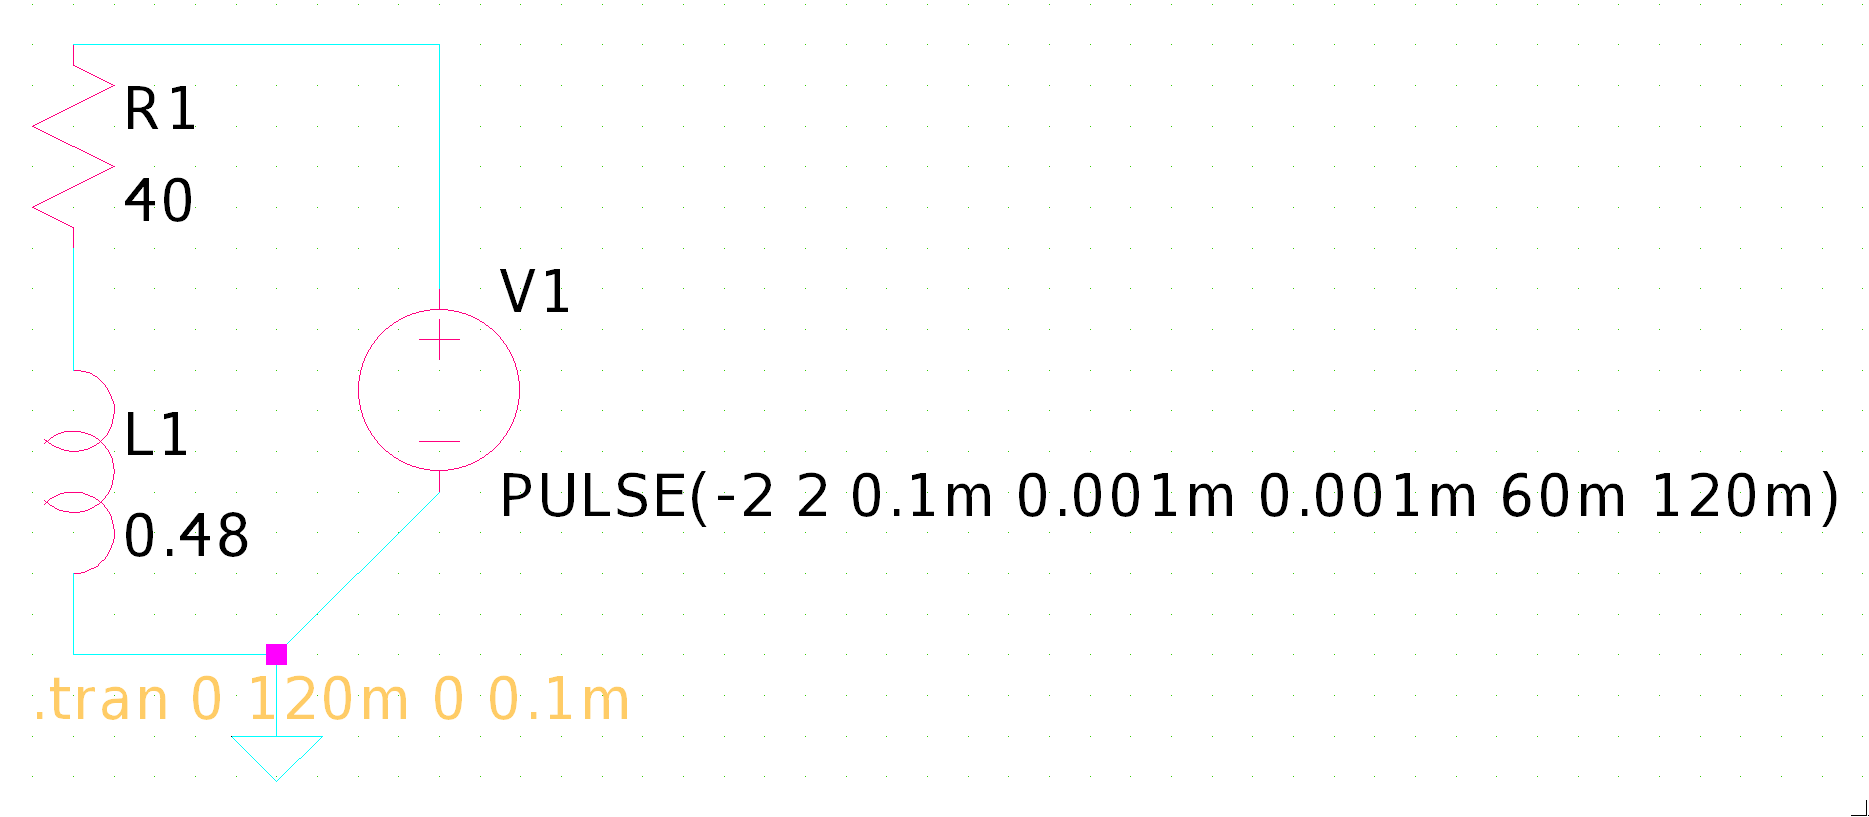
\includegraphics[width=1\textwidth]{./data/rl-schema.png}
	\caption{Схема замещения RL-цепи в LTspice.}
\end{figure}

\subsubsection{Расчётные формулы и расчёты}
\begin{enumerate}
	\item Определение топологии цепи:
	      \begin{align*}
		      p^*           & = 6 \, (\text{общее количество ветвей}),                                    \\
		      p_{\text{ит}} & = 1 \, (\text{количество ветвей с источниками тока}),                       \\
		      p             & = p^* - p_{\text{ит}} = 6 - 1 = 5 \, (\text{количество неизвестных токов}), \\
		      q             & = 4 \, (\text{количество узлов}),                                           \\
		      l             & = q - 1 = 4 - 1 = 3 \, (\text{количество узловых напряжений})
	      \end{align*}

	\item Произвольно обозначим $p$ неизвестных токов и $l$ узловых напряжений, где узел с номером "0" — заземлённый. От оставшихся незаземленных узлов направляем узловые напряжения к заземленному узлу:
	      \begin{figure}[H]
	\centering
	\begin{circuitikz}[american, scale=1.4]

		\draw
		(0,0)
		to[R, l=$R_3$, i=$I_3$] (10,0)
		-- (10, -3)
		to[short, *-] (10, -3);

		\draw
		(10, -3)
		to[R, l_=$R_5$, i=$I_5$] (7.5, -3)
		to[I, l=$E_5$] (5, -3)
		to[short, *-] (5, -3)
		to[R, l=$R_2$, i=$I_2$] (2.5, -3)
		to[I, l_=$E_2$] (0, -3);

		\draw
		(0,0)
		-- (0,-3)
		to[short, *-] (0, -3)
		to[R, l=$R_1$, i_=$I_1$] (5, -6);

		\draw
		(5, -3)
		to[R, l=$R_4$, i=$I_4$] (5, -6);

		\draw (5, -6) -- (7.15, -4.7);
		\draw (7.85, -4.3) -- (10, -3);
		\draw[rotate around={-52:(7.5,-4.5)}]
		(7.5,-4.5) circle(0.4cm)
		(7.5,-4.45) edge[thick, -{Straight Barb[length=2mm]}] (7.5, -4.44)
		(7.5,-4.35) edge[thick, -{Straight Barb[length=2mm]}] (7.5, -4.34)
		node at (8.25, -4.5) {$J_6$};

		\draw (0, -3) node[draw, circle, fill=blue!10, scale=0.8] {\textcolor{blue}{1}};
		\draw (5, -3) node[draw, circle, fill=blue!10, scale=0.8] {\textcolor{blue}{2}};
		\draw (10, -3) node[draw, circle, fill=blue!10, scale=0.8] {\textcolor{blue}{3}};
		\draw (5, -6) node[draw, circle, fill=blue!10, scale=0.8] {\textcolor{blue}{0}};

		\draw[red, thick, dashed, ->]
		(0, -3.4) .. controls (0, -5) and (2.5, -6.5) .. (4.5, -6.1)
		node[midway, left, xshift=-0.2cm, red] {$U_{10}$};

		\draw[red, thick, dashed, ->] (4.7, -3.3) arc[start angle=130, end angle=230, radius=1.5] node[midway, left, red] {$U_{20}$};

		\draw[red, thick, dashed, ->]
		(10, -3.4) .. controls (10, -5) and (7.5, -6.5) .. (5.5, -6.1)
		node[midway, right, xshift=0.4cm, red] {$U_{30}$};

		\draw (5, -6.25) node[ground] {};


	\end{circuitikz}
	\caption{Схема электрической цепи с узлами, узловыми напряжениями и токами}
\end{figure}


	\item Составим систему уравнений на основе узловых напряжений. Для этого используем проводимости всех ветвей, за исключением ветвей с источниками тока. Собственные проводимости узлов — это сумма проводимостей всех ветвей, сходящихся в данный узел. В правой части уравнений находятся «узловые токи», которые включают алгебраическую сумму токов и источников энергии, действующих в ветвях узла.
	      \[
		      \begin{cases}
			      g_{11} U_{10} - g_{12} U_{20} - g_{13} U_{30} = J_{11},  \\
			      -g_{21} U_{10} + g_{22} U_{20} - g_{23} U_{30} = J_{22}, \\
			      -g_{31} U_{10} - g_{32} U_{20} + g_{33} U_{30} = J_{33}.
		      \end{cases}
	      \]

	      где \( g_{km} = g_{mk} \, (k=1\ldots l, \, m=1\ldots l, \, k \neq m) \) — общие проводимости, которые являются суммой проводимостей всех ветвей, расположенных между узлами \( k \) и \( m \) (кроме проводимости ветвей с источником тока). \( g_{kk} \) — собственные проводимости, которые представляют собой сумму проводимостей всех ветвей, сходящихся в узле \( k \) (кроме ветвей с источником тока). \( J_{kk} \) — это узловые токи, обусловленные наличием источников энергии в узлах.

	\item Запишем систему уравнений с подстановкой проводимостей и ЭДС:

	      \[
		      \begin{cases}
			      \left( \frac{1}{R_1} + \frac{1}{R_2} + \frac{1}{R_3} \right) U_{10} - \left( \frac{1}{R_2} \right) U_{20} - \left( \frac{1}{R_3} \right) U_{30} = -\frac{E_2}{R_2},                    \\
			      -\left( \frac{1}{R_2} \right) U_{10} + \left( \frac{1}{R_2} + \frac{1}{R_4} + \frac{1}{R_5} \right) U_{20} - \left( \frac{1}{R_5} \right) U_{30} = -\frac{E_2}{R_2} + \frac{E_5}{R_5}, \\
			      -\left( \frac{1}{R_3} \right) U_{10} - \left( \frac{1}{R_5} \right) U_{20} + \left( \frac{1}{R_3} + \frac{1}{R_5} \right) U_{30} = -\frac{E_5}{R_5} + J_6.
		      \end{cases}
	      \]

	\item Подставим численные значения для сопротивлений, тока и ЭДС:

	      \[
		      \begin{cases}
			      \left( \frac{1}{8} + \frac{1}{6} + \frac{1}{7} \right) U_{10} - \left( \frac{1}{6} \right) U_{20} - \left( \frac{1}{7} \right) U_{30} = -\frac{34.5}{6},                \\
			      -\left( \frac{1}{6} \right) U_{10} + \left( \frac{1}{6} + \frac{1}{5} + \frac{1}{7} \right) U_{20} - \left( \frac{1}{7} \right) U_{30} = -\frac{34.5}{6} + \frac{7}{7}, \\
			      -\left( \frac{1}{7} \right) U_{10} - \left( \frac{1}{7} \right) U_{20} + \left( \frac{1}{7} + \frac{1}{7} \right) U_{30} = \frac{7}{7} + 1.95.
		      \end{cases}
	      \]

	\item Решая данную систему, получаем значения узловых напряжений:

	      \[
		      U_{10} = 16.927 \, \text{В}, \quad U_{20} = -0.332 \, \text{В}, \quad U_{30} = 11.623 \, \text{В}.
	      \]

	\item Опреледение искомых токов через узловые напряжения:

	      \[
		      \begin{gathered}
			      I_1 = \frac{\varphi_1 - \varphi_0}{R_1} = \frac{U_{10}}{R_1} = \frac{16.927}{8} = 2.116 \, \text{А} \\
			      \\[-0.5em]
			      I_4 = \frac{\varphi_2-\varphi_0}{R_4} = \frac{U_{20}}{R_4} = \frac{-0.332}{2} = -0.166 \, \text{А} \\
		      \end{gathered}
	      \]

	      \[
		      \begin{gathered}
			      I_2 = \frac{\varphi_2 - \varphi_1 + E_2}{R_2} = \frac{(\varphi_2 -\varphi_0) - (\varphi_1 - \varphi_0) + E_2}{R_2} = \frac{(U_{20}-U_{10}+E_2)}{R_2} = \\
			      = \frac{-0.332-16.927+34.5}{6} = 2.874 \, \text{А} \\
			      I_3 = \frac{\varphi_1 - \varphi_3}{R_3} = \frac{(\varphi_1 -\varphi_0) - (\varphi_3 - \varphi_0)}{R_3} = \frac{U_{10}-U_{30}}{R_3} = \\
			      = \frac{16.927-11.623}{7} = 0.758 \, \text{А} \\
			      I_5 = \frac{\varphi_3-\varphi_2+E_5}{R_5} = \frac{(\varphi_3-\varphi_0)-(\varphi_2-\varphi_0)+E_5}{R_5} = \frac{U_{30}-U_{20}+E_5}{R_5} = \\
			      = \frac{11.623+0.332+7}{7} = 2.708 \, \text{А} \\
		      \end{gathered}
	      \]
\end{enumerate}


\subsubsection{График переходного процесса в RL-цепи}
% lab2-2.txt graph structure:
% time	V(n001)	V(n002)	I(R1)

\begin{figure}[H]
	\centering
	\begin{tikzpicture}[scale=0.88]
		\begin{axis}[
				width=17cm, height=12cm,
				xlabel={Time [ms]},    % X-axis label
				ylabel={Voltage [V]},    % Y-axis label
				grid=major,           % Enable grid
				legend style={at={(0.857,0.95)}, anchor=north west}, % Legend position
				thick,                % Line thickness
				xmin=0, xmax=120,    % X-axis range
				ymin=-4, ymax=4,      % Y-axis range
				axis y line=left,
				axis x line=bottom,
				label style={font=\small},
				tick label style={font=\small},
				major tick length=0.2cm,
				ytick style={thick, black},
				xtick style={thick, black},
				ytick={-3.2, -2.4, -1.6, -0.8, 0, 0.8, 1.6, 2.4, 3.2},
				extra y ticks={-4, 4},
				extra y tick style={tick style={opacity=0}},
				x unit=0.001,
			]

			% Plot V(n001)
			\addplot[
				color=red,
				thick,
			] table [x expr=\thisrowno{0}*1000, y index=1, col sep=space] {./data/lab2-2.txt};
			\addlegendentry{$E$}

			% Plot V(n002)
			\addplot[
				color=green,
				thick,
			] table [x expr=\thisrowno{0}*1000, y index=2, col sep=space] {./data/lab2-2.txt};
			\addlegendentry{$U_L$}

			\addplot[color=black, only marks, mark=*, mark size=1pt] coordinates {(0, 4)};
			\node[anchor=west] at (axis cs:0,3.85) {\scriptsize $U_L(0+) = 4 \, V$};

			\addplot[color=black, only marks, mark=*, mark size=1.5pt] coordinates {(60, 0.027)};
			\node[anchor=east] at (axis cs:61,-0.15) {\scriptsize $0.027 \, V = U_L(\infty)$};
			\draw[dashed, grey, very thin] (axis cs:0, 0.027) -- (axis cs:60, 0.027);

		\end{axis}

		% Secondary axis for Current
		\begin{axis}[
				width=17cm, height=12cm,
				xmin=0, xmax=120,    % X-axis range (same as for Voltage)
				ymin=-50, ymax=50,  % Y-axis range for Current
				axis y line=right,         % Place this axis on the right for Current
				axis x line=none,
				thick,
				ylabel={Current [mA]}, % Y-axis label for Current
				label style={font=\small},
				tick label style={font=\small},
				major tick length=0.2cm,
				ytick style={thick, black},
				ytick={-40, -30, -20, -10, 0, 10, 20, 30, 40},
				extra y ticks={-50, 50},
				extra y tick style={tick style={opacity=0}},
				legend style={at={(0.96,0.82)}, anchor=north east},
			]
			% Plot I(R1)
			\addplot[color=blue, thick] table [x expr=\thisrowno{0}*1000, y expr=\thisrowno{3}*1000, col sep=space] {./data/lab2-2.txt};
			\addlegendentry{$I$}

			\addplot[color=black, only marks, mark=*, mark size=1.5pt] coordinates {(120, -49.324)};
			\node[
				anchor=east,
				font=\scriptsize
			] at (axis cs:121,-47) {$-49.324\, \text{mA} = I(0+)$};

			\addplot[color=black, only marks, mark=*, mark size=1.5pt] coordinates {(60.1, 49.325)};
			\draw[dashed, grey, very thin] (axis cs:60, 49.3) -- (axis cs:120, 49.3);
			\node[anchor=west] at (axis cs:60.1,47) {\scriptsize $I(\infty) = 49.325 \, mA$};
		\end{axis}
	\end{tikzpicture}
\end{figure}


\subsubsection{Таблица результатов 4.3}
Таблица 4.3 содержит эксперементальные и расчётные результаты длительности переходного процесса в RL-цепи, а также тока и напряжения в момент коммутации и в установившемся режиме.

\begin{table}[h]
	\centering
	\resizebox{\textwidth}{!}{
		\begin{tabular}{|c|c|c|c|c|c|c|c|}
			\hline
			$R$ [Ом]            & $L$ [мГн]            & Тип данных & $I(0+)$ [мА] & $I(\infty)$ [мА] & $U_L(0+)$ [В] & $U_L(\infty)$ [В] & $\tau$ [мкс] \\
			\hline
			\multirow{2}{*}{40} & \multirow{2}{*}{480} & эксп.      & -49.324      & 49.325           & 4             & 0.027             & 12\,143      \\
			\cline{3-8}
			                    &                      & расч.      & -50          & 50               & 4             & 0                 & 12\,000      \\ \hline
		\end{tabular}
	}
	\caption{Результаты измерений и расчётов для RC-цепи}
\end{table}



% -------------------------------


\subsection{Выводы по первой части}

В результате выполнения первой части лабораторной работы я исследовал переходные процессы в RC и RL цепях и выяснил, что постоянная времени \(\tau\), равная 12 мс, описывает скорость изменения токов и напряжений. За это время величины изменяются примерно на 63\% от максимального значения. Экспоненциальный характер графиков обусловлен свойствами дифференциальных уравнений, описывающих процессы зарядки и разрядки конденсатора, а также роста и спада тока через индуктивность.

Экспериментальные значения \(\tau\), полученные аппроксимацией на основе ближайших точек графика, экспортированных из LTSpice, составили 12.144 мс для RC-цепи и 12.143 мс для RL-цепи, что близко к расчётным 12 мс. Отклонение менее 1.2\% говорит о высокой точности эксперимента. Кроме того, отклонения других величин (токов и напряжений в момент коммутации и в установившемся режиме) также оказались небольшими: ток в RC-цепи составил 99.996 мА против расчётных 100 мА, а напряжение на катушке в RL-цепи было 0.027 В против теоретических 0 В в установившемся режиме. Эти результаты показывают, что эксперименты подтвердили теоретические модели с минимальными расхождениями.

При этом я заметил, что в каждом эксперименте ток и напряжение достигают половины своих амплитуд \(t_{0.5}\) за разное время (разница составляет около 4–6 мс). Это объясняется тем, что конденсатор и катушка сопротивляются резким изменениям: электростатическое поле конденсатора замедляет изменение напряжения на нём, так как при накоплении заряда на обкладках возникает сильное электростатическое поле, которое требует времени для изменения (перемещения зарядов через цепь). Катушка же сопротивляется изменению тока за счёт магнитного поля, которое индуцирует ЭДС (самоиндукция), противодействующую изменению тока (закон Ленца).

Также в будущем можно было бы учесть полное сопротивление (импеданс) катушки и конденсатора для более точного моделирования, но в наших опытах эти эффекты не рассматривались (пренебрегали реактивными сопротивлениями).


% -------------------------------

\section*{Часть 2}
\addcontentsline{toc}{section}{Часть 2}
\stepcounter{section}
\subsection{Введение}

Чтобы понять, при каком значении сопротивления в цепи будет наблюдаться \textbf{колебательный} процесс, а при каком \textbf{апериодический}, нужно найти характеристическое сопротивление, которое для цепи второго порядка определяется как:

\[
	p = \sqrt{\frac{L}{C}} = \sqrt{\frac{0,48}{300 \cdot 10^{-6}}} = 40 \, \text{Ом}
\]

На основе этой величины можно понять какой будет процесс: Если $R > p$, то затухания колебаний ускоряются и энергия системы не возвращается в исходное состояние, если $R = 2 \cdot p$ -- это критический момент, когда процесс перестаёт быть апериодическим, но возвращается в равновесное состояние без колебаний, а при $R < 2 \cdot p$ энергия будет поочерёдно передаваться между индуктивностью и ёмкостью, вызывая затухающие колебания.

Таким образом, при $R = 4 \cdot p = 4 \cdot 40 = 160 \, \text{Ом}$ наблюдается \textit{апериодический} процесс, а при $R = \frac{p}{2} = \frac{40}{2} = 20 \, \text{Ом}$ -- \textit{колебательный}.


% -------------------------------


\subsection{Исследование апериодического процесса}

\subsubsection{Схема исследуемой цепи}
На рисунке 3 представлена схема замещения цепи второго порядка, состоящей из генератора прямоугольного напряжения с резистивной, ёмкостной и индуктивной нагрузками, созданная в приложении LTspice.

\begin{figure}[H]
	\centering
	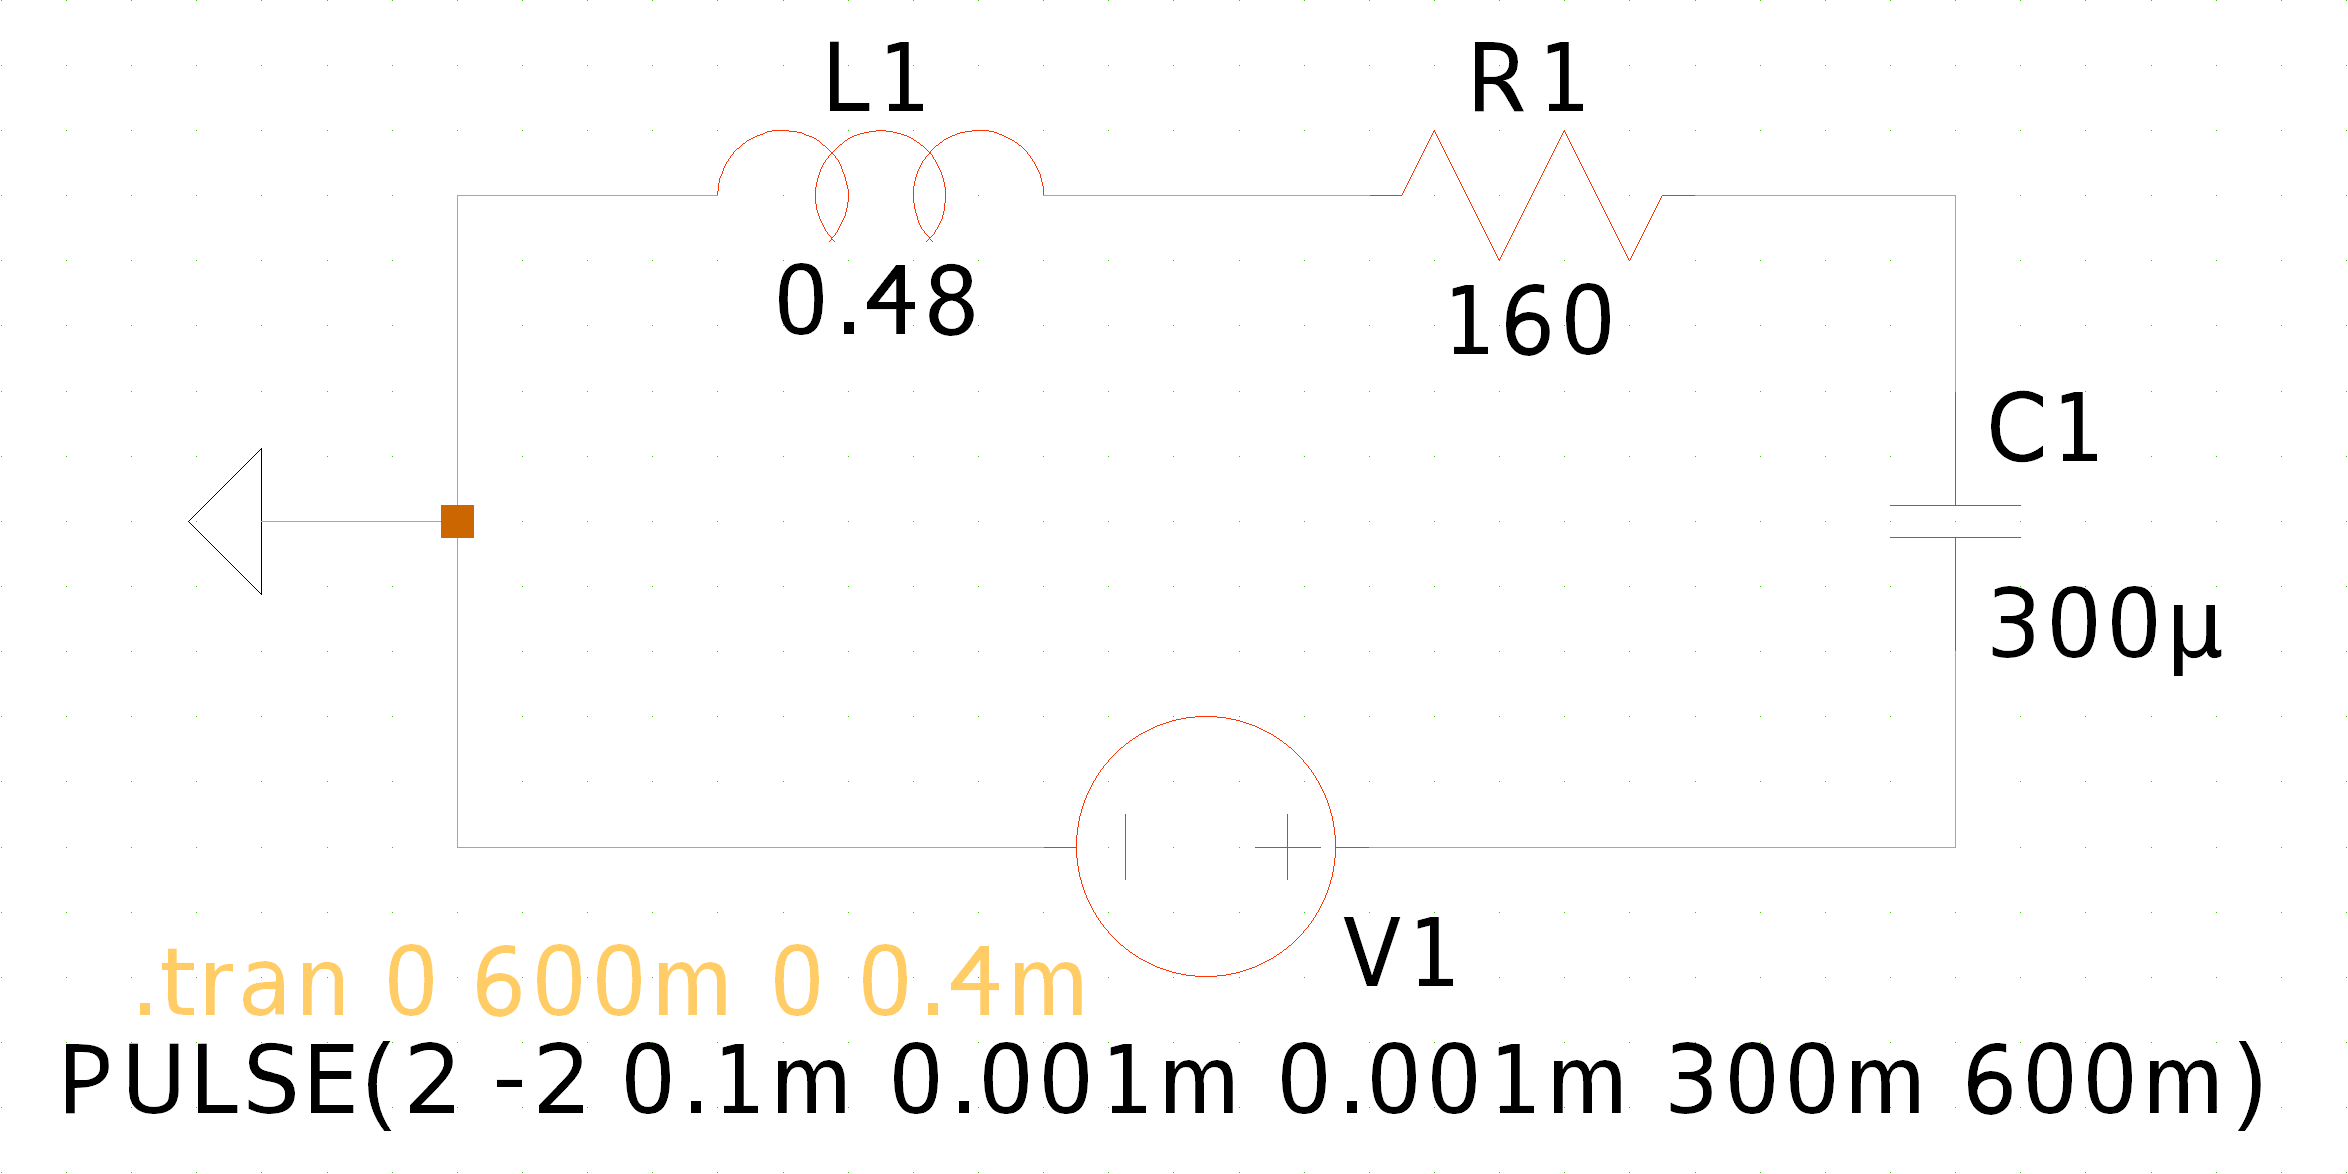
\includegraphics[width=1\textwidth]{./data/rcl_1-schema.png}
	\caption{Схема замещения RCL-цепи в LTspice.}
\end{figure}

\subsubsection{Расчётные формулы и расчёты}

Значение времени переходного процесса \( t_{0.5} \) определяется как время, за которое напряжение на конденсаторе достигает половины своего установившегося значения. Постоянная времени \( \tau \) определяется как:

\[
	\tau = \frac{t_{0.5}}{\ln 2}
\]

\textbf{Вычисление постоянной времени \( \tau \):}

\[
	\tau = \frac{t_{0.5}}{\ln 2} = \frac{8.41833 \, \text{мс}}{0.69314718} = 12.144 \, \text{мс}
\]

\subsubsection{График апериодического переходного процесса}
% time	V(N003,N001)  V(n002)  V(n003)  I(C1)

\begin{figure}[H]
	\centering
	\begin{tikzpicture}[scale=0.88]
		\begin{axis}[
				width=17cm, height=12cm,
				xlabel={Time [ms]},    % X-axis label
				ylabel={Voltage [V]},    % Y-axis label
				grid=major,           % Enable grid
				legend style={at={(0.857,0.95)}, anchor=north west}, % Legend position
				thick,                % Line thickness
				xmin=0, xmax=600,    % X-axis range
				ymin=-4, ymax=4,      % Y-axis range
				axis y line=left,
				axis x line=bottom,
				label style={font=\small},
				tick label style={font=\small},
				major tick length=0.2cm,
				ytick style={thick, black},
				xtick style={thick, black},
				ytick={-3.2, -2.4, -1.6, -0.8, 0, 0.8, 1.6, 2.4, 3.2},
				extra y ticks={-4, 4},
				extra y tick style={tick style={opacity=0}},
				x unit=0.001,
			]

			% Plot V(n001)
			\addplot[
				color=red,
				thick,
			] table [x expr=\thisrowno{0}*1000, y index=3, col sep=space] {./data/lab2-3.txt};
			\addlegendentry{$E$}

			% Plot V(n002)
			\addplot[
				color=magenta,
				thick,
			] table [x expr=\thisrowno{0}*1000, y index=1, col sep=space] {./data/lab2-3.txt};
			\addlegendentry{$U_L$}
			%
			% \addplot[color=black, only marks, mark=*, mark size=1pt] coordinates {(0, 4)};
			% \node[anchor=west] at (axis cs:0,3.85) {\scriptsize $U_L(0+) = 4 \, V$};
			%
			% \addplot[color=black, only marks, mark=*, mark size=1.5pt] coordinates {(60, 0.027)};
			% \node[anchor=east] at (axis cs:61,-0.15) {\scriptsize $0.027 \, V = U_L(\infty)$};
			% \draw[dashed, grey, very thin] (axis cs:0, 0.027) -- (axis cs:60, 0.027);

			% Plot V(n002)
			\addplot[
				color=green,
				thick,
				% nodes near coords,
				% mark=*,
				% every node near coord/.append style={font=\tiny, black}
			] table [x expr=\thisrowno{0}*1000, y index=2, col sep=space] {./data/lab2-3.txt};
			\addlegendentry{$U_c$}

			% \draw[dashed,grey,very thin] (axis cs:120,1.972884) -- (axis cs:60.1,1.972884);
			% \addplot[color=black, only marks, mark=*, mark size=1.5pt] coordinates {(60.1,1.972884)};
			% \node[anchor=west] at (axis cs:60.1,1.872884) {\scriptsize $U_c(\infty) = 1.973 \, V$};
			%
			% \draw[dashed,grey,very thin] (axis cs:120,-1.973) -- (axis cs:120, -1.973)
			% \addplot[color=black, only marks, mark=*, mark size=1.5pt] coordinates {(120, -1.973)};
			% \node[anchor=east] at (axis cs:121,-1.82) {\scriptsize $ -1.973 \, V = U_c(0+)$};


		\end{axis}

		% Secondary axis for Current
		\begin{axis}[
				width=17cm, height=12cm,
				xmin=0, xmax=600,    % X-axis range (same as for Voltage)
				ymin=-80, ymax=80,  % Y-axis range for Current
				axis y line=right,         % Place this axis on the right for Current
				axis x line=none,
				thick,
				ylabel={Current [mA]}, % Y-axis label for Current
				label style={font=\small},
				tick label style={font=\small},
				major tick length=0.2cm,
				ytick style={thick, black},
				ytick={-70, -60, -50, -40, -30, -20, -10, 0, 10, 20, 30, 40, 50, 60, 70},
				extra y ticks={-80, 80},
				extra y tick style={tick style={opacity=0}},
				legend style={at={(0.961,0.765)}, anchor=north east},
			]
			% Plot I
			\addplot[
				color=cyan,
				thick,
			] table [x expr=\thisrowno{0}*1000, y expr=\thisrowno{4}*1000, col sep=space] {./data/lab2-3.txt};
			\addlegendentry{$I$}

			% \addplot[color=black, only marks, mark=*, mark size=1.5pt] coordinates {(120, -49.324)};
			% \node[
			% 	anchor=east,
			% 	font=\scriptsize
			% ] at (axis cs:121,-47) {$-49.324\, \text{mA} = I(0+)$};
			%
			% \addplot[color=black, only marks, mark=*, mark size=1.5pt] coordinates {(60.1, 49.325)};
			% \draw[dashed, grey, very thin] (axis cs:60, 49.3) -- (axis cs:120, 49.3);
			% \node[anchor=west] at (axis cs:60.1,47) {\scriptsize $I(\infty) = 49.325 \, mA$};
		\end{axis}
	\end{tikzpicture}
\end{figure}


\subsubsection{Таблица результатов 4.4}


% -------------------------------


\subsection{Исследование колебательного процесса}

\subsubsection{Схема исследуемой цепи}
На рисунке 4 представлена схема замещения генератора прямоугольного напряжения с резистивной, ёмкостной и индуктивной нагрузками, созданная в приложении LTspice.

\begin{figure}[H]
	\centering
	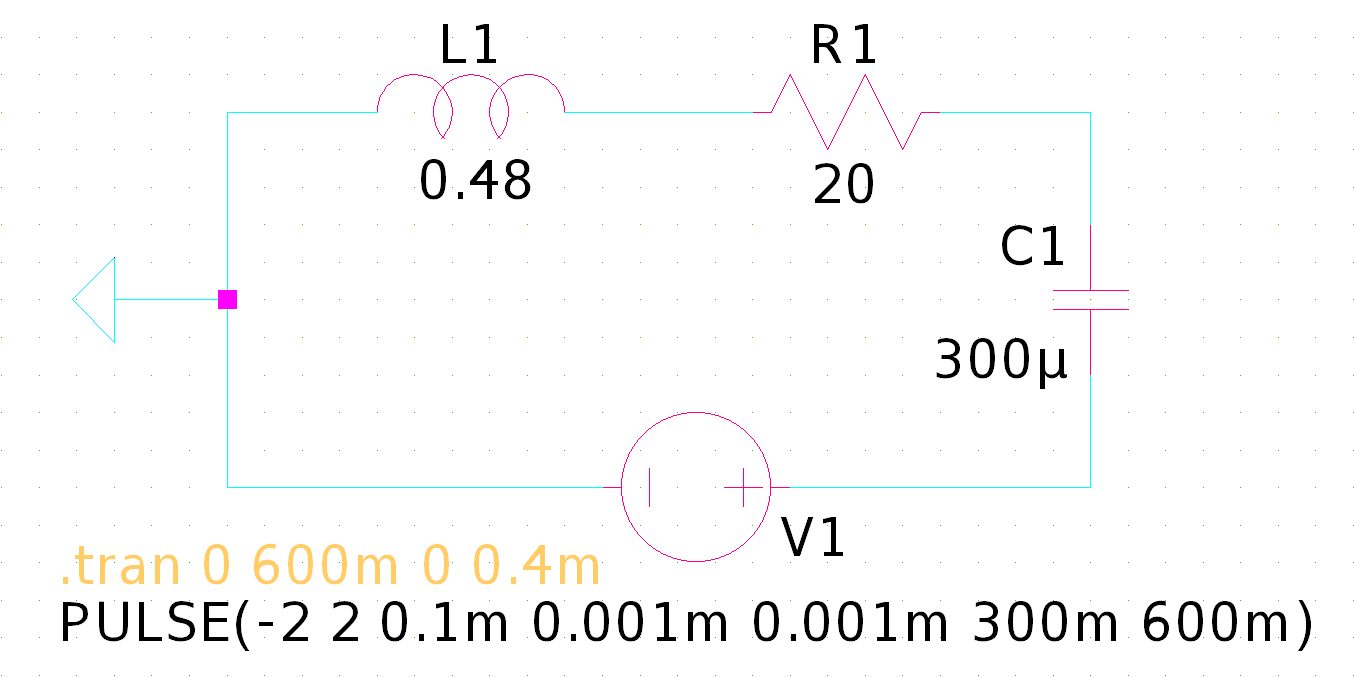
\includegraphics[width=0.96\textwidth]{./data/rcl_2-schema.png}
	\caption{Схема замещения RCL-цепи в LTspice.}
\end{figure}

\subsubsection{Расчётные формулы и расчёты}

\subsubsection{График колебательного переходного процесса}
% time	V(N003,N001)  V(n002)  V(n003)  I(C1)

\begin{figure}[H]
	\centering
	\begin{tikzpicture}[scale=0.88]
		\begin{axis}[
			width=17cm, height=12cm,
			xlabel={Время [мс]},
			ylabel={Напряжение [В]},
			grid=major,           % Enable grid
			legend style={at={(0.857,0.95)}, anchor=north west}, % Legend position
			thick,                % Line thickness
			xmin=0, xmax=600,    % X-axis range
			ymin=-4, ymax=4,      % Y-axis range
			axis y line=left,
			axis x line=bottom,
			label style={font=\small},
			tick label style={font=\small},
			major tick length=0.2cm,
			ytick style={thick, black},
			xtick style={thick, black},
			ytick={-3, -2, -1, 0, 1, 2, 3},
			extra y ticks={-4, 4},
			extra y tick style={tick style={opacity=0}},
			x unit=0.001,
			]

			% Plot V(n001)
			\addplot[
				color=teal,
				line width=1.2pt,
			] table [x expr=\thisrowno{0}*1000, y index=3, col sep=space] {./data/lab2-4.txt};
			\addlegendentry{$E$}

			% Plot V(n002)
			\addplot[
				color=orange,
				line width=1.2pt,
			] table [x expr=\thisrowno{0}*1000, y index=1, col sep=space] {./data/lab2-4.txt};
			\addlegendentry{$U_c$}
			%
			% \addplot[color=black, only marks, mark=*, mark size=1pt] coordinates {(0, 4)};
			% \node[anchor=west] at (axis cs:0,3.85) {\scriptsize $U_L(0+) = 4 \, V$};
			%
			% \addplot[color=black, only marks, mark=*, mark size=1.5pt] coordinates {(60, 0.027)};
			% \node[anchor=east] at (axis cs:61,-0.15) {\scriptsize $0.027 \, V = U_L(\infty)$};
			% \draw[dashed, grey, very thin] (axis cs:0, 0.027) -- (axis cs:60, 0.027);

			% Plot V(n002)
			\addplot[
				color=magenta,
				line width=1.2pt,
				% nodes near coords,
				% mark=*,
				% every node near coord/.append style={font=\tiny, black}
			] table [x expr=\thisrowno{0}*1000, y index=2, col sep=space] {./data/lab2-4.txt};
			\addlegendentry{$U_L$}

			% \draw[dashed,grey,very thin] (axis cs:120,1.972884) -- (axis cs:60.1,1.972884);
			% \addplot[color=black, only marks, mark=*, mark size=1.5pt] coordinates {(60.1,1.972884)};
			% \node[anchor=west] at (axis cs:60.1,1.872884) {\scriptsize $U_c(\infty) = 1.973 \, V$};
			%
			% \draw[dashed,grey,very thin] (axis cs:120,-1.973) -- (axis cs:120, -1.973)
			% \addplot[color=black, only marks, mark=*, mark size=1.5pt] coordinates {(120, -1.973)};
			% \node[anchor=east] at (axis cs:121,-1.82) {\scriptsize $ -1.973 \, V = U_c(0+)$};


		\end{axis}

		% Secondary axis for Current
		\begin{axis}[
			width=17cm, height=12cm,
			xmin=0, xmax=600,    % X-axis range (same as for Voltage)
			ymin=-80, ymax=80,  % Y-axis range for Current
			axis y line=right,         % Place this axis on the right for Current
			axis x line=none,
			thick,
			line width=1.3pt,
			ylabel={Ток [мА]},
			label style={font=\small},
			tick label style={font=\small},
			major tick length=0.2cm,
			ytick style={thick, black},
			ytick={-60, -40, -20, 0, 20, 40, 60},
			extra y ticks={-80, 80},
			extra y tick style={tick style={opacity=0}},
			legend style={at={(0.961,0.765)}, anchor=north east},
			]
			% Plot I
			\addplot[
				color=cyan,
				line width=1.2pt,
			] table [x expr=\thisrowno{0}*1000, y expr=\thisrowno{4}*1000, col sep=space] {./data/lab2-4.txt};
			\addlegendentry{$I$}

			% \addplot[color=black, only marks, mark=*, mark size=1.5pt] coordinates {(120, -49.324)};
			% \node[
			% 	anchor=east,
			% 	font=\scriptsize
			% ] at (axis cs:121,-47) {$-49.324\, \text{mA} = I(0+)$};
			%
			% \addplot[color=black, only marks, mark=*, mark size=1.5pt] coordinates {(60.1, 49.325)};
			% \draw[dashed, grey, very thin] (axis cs:60, 49.3) -- (axis cs:120, 49.3);
			% \node[anchor=west] at (axis cs:60.1,47) {\scriptsize $I(\infty) = 49.325 \, mA$};
		\end{axis}
	\end{tikzpicture}
\end{figure}


\subsubsection{Таблица результатов 4.5}

\subsection{Выводы по второй части}


% % -------------------------------
%
% \section*{Выводы по работе}
% \addcontentsline{toc}{section}{Выводы по работе}
% \stepcounter{section}
%
% Вывод по работе

\end{document}
